\documentclass[a4paper]{article}

\usepackage[margin=1.0in]{geometry}
\usepackage{biblatex}
\usepackage{graphics}
\usepackage{graphicx}
\usepackage{subcaption}

\title{Short Term Scholar Weekly Progress Report 6}
\author{Ufuk Bombar}
\date{August 18, 2019}

\addbibresource{bib.bib}

\begin{document}

    \maketitle{}
    The goal of this week is to learn more on graphs and other possible applications and start implementation.

    \paragraph{}
    On Monday, I started to read an article, covering the methods of optimizations for graph traversal algorithms\cite{graph}. The article divides the graph traversal into two sub-problems. First is the \textit{static routing} and secondly, \textit{time dependent routing}. The \textit{static routing} covers all the optimizations for graphs that have static edges. For example, a local internet network can be represented as a static network. Because the weight of the edges does not depend on time. On the other hand, a road network mostly classified as a time-dependent network since the weight of the edges depends on the traffic and as a result time. I acknowledged that there are many methods for pre-processing. For example, in static routing, the graph is optimized by running a method before any search queue. This method groups the nodes into chunks. So that search queues can be processed starting from high level to low level. This method in general named \textit{node contraction}. Figure \ref{fig:nodecontraaction} shows this method visually. However, a bigger problem rests on the \textit{time dependent routing}. Since the weight of the edges constantly changing the optimizations are harder to achieve and they are dependent to the shape of the graph. After covering the paper, I decided to make a traffic simulator application. I cogitated on basic features and implementation requirements. Rest of my time I work on setting up the environment for development.
    
    \paragraph{}
	On Tuesday, I work on the format of \textit{analysis report}. Most of my time spent on learning to format on latex. After I finish the formatting, I started to add functional and non-functional requirements to the analysis report. In the middle of the report, I asked for feedback to Mr. Altınakar. We decided to move forward with another application that requires more interaction with raster files. He also gave me some articles to read. They were about extracting information from elevation data\cite{ex1, ex4, ex5} and calculation of road lines for minimal earthwork\cite{earthwork}. I mostly interested in earthwork. I imagined a program that finds the road line for minimum earthwork. But before that, I started to do background research about \textit{watersheds}.
    
    \paragraph{}
    On Wednesday, I read the last section of chapter 11 and finally finished it. By that, I learned possible computations I can do on raster files. I decided to write a small program for creating an elevation map from my vector file. First, I created an empty raster file, then I created a vector file that contains polygons of different elevation attributes. After that, I projected the vector to a raster file. But to make a plot the resolution was too high. Therefore, I re-sampled it to a lower resolution by using bilinear filtering. This method allows to re-sample an image while smoothing the sharp edges\cite{geobook}. Then, I achieved an artificial elevation map made by a vector file. Lastly, I used \textit{matplotlib} to create a 3d graph of the elevation map. The 3d plot shown in figure \ref{fig:plot}.
    
    \paragraph{}
    On Tuesday, I continued my readings. I learned \textit{steam order}. \textit{Steam order} is a numbering system of the steam branches that are used in different scenarios and algorithms. However, the numbering of branches varies. A most common one, \textit{Strahler steam order} only allows the rank of the branch to be incremented if the sub-branches have the same ranks. Figure \ref{fig:strahler} shows the numbering process visually. Another method is the \textit{Shreve steam order} shown in figure \ref{fig:shreve} which calculates the rank of a branch by adding other connected branches. It is important to note that the rank does not necessarily mean size. These ranks can be used for different purposes.
    
    \begin{figure}
        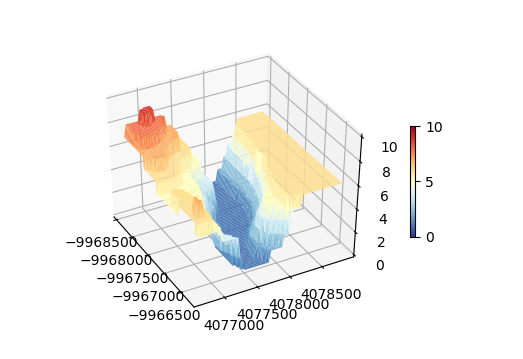
\includegraphics[width=\linewidth]{plot3.png}
        \caption{Plot of elevation map.}
        \label{fig:plot}
    \end{figure}

    \begin{figure}
        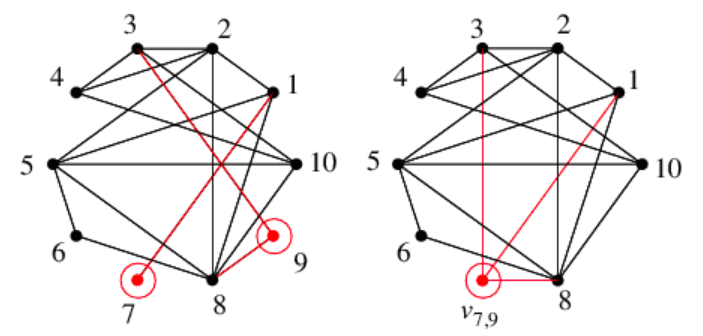
\includegraphics[width=\linewidth]{out.png}
        \caption{Node contraction \cite{wolfram}.}
        \label{fig:nodecontraaction}
    \end{figure}

    \begin{figure}[h!]
        \centering
        \begin{subfigure}[b]{0.4\linewidth}
            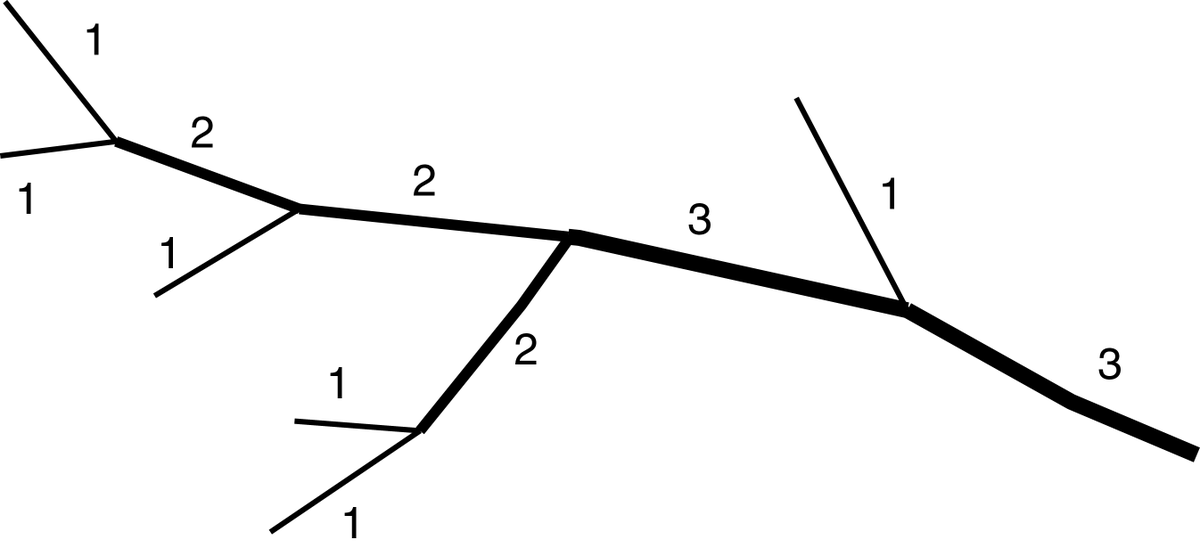
\includegraphics[width=\linewidth]{strahler.png}
            \caption{Strahler steam order.}
            \label{fig:strahler}
        \end{subfigure}
        \begin{subfigure}[b]{0.4\linewidth}
            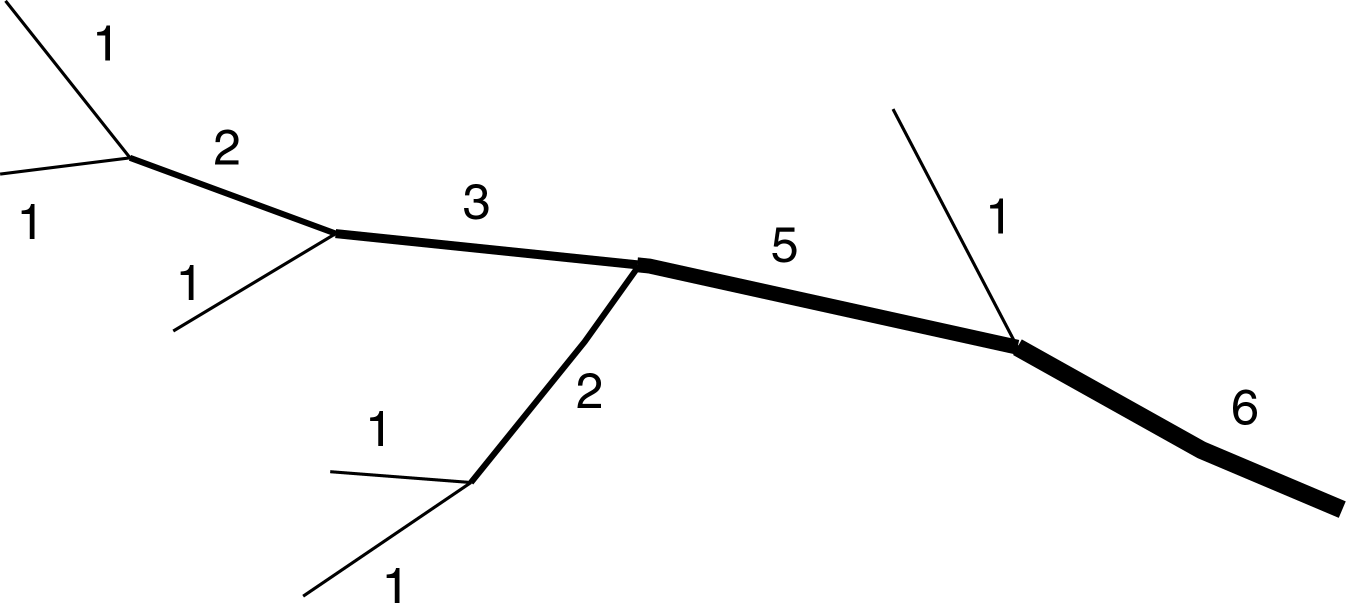
\includegraphics[width=\linewidth]{shreve.png}
            \caption{Shreve steam order.}
            \label{fig:shreve}
        \end{subfigure}
        \caption{Comparison of Shrahler and Shreve steam order.}
    \end{figure}

    \printbibliography    
\end{document}